\chapter{Appendix} \label{appendix}
\section{Hematopoiesis}
The production of all types of blood cells including the formation, development, maturation, and differentiation of blood cells is called hematopoiesis. Its purpose is to ensure the constant daily production of mature cells of the peripheral blood both in healthy condition and in response to particular situations of increased demand, such as in the presence of infection or blood loss. The hematopoiesis is supported by a small number of primitive cells called \textit{Haematopoietic Stem Cells} (\acs{HSC}s) or \textit{haemocytoblasts}, characterized by the ability of self-renewing, namely the ability to generate cells identical to themselves. At the same time, the HSCs are pluripotent, having the potential to develop into all types of blood cells. Hematopoiesis occurs in bone marrow, where the HSCs are present in the ratio of one stem cell for every 1.000 non-stem cell elements. It is why the cause and effect of haematologic disease are usually rooted in the bone marrow. Usually, only healthy, mature or nearly mature cells are released into the bloodstream, but certain circumstances can induce the bone marrow to release immature and abnormal cells into the circulation. The predominance of immature cells noted in a complete blood count is indicative of infections, inflammations, and other severe illnesses. It is also the reason why it is essential to analyze the whole hematopoietic process, being able to recognize inside the blood smears any cell type at any stage of maturation. The HSCs give rise to mature cells, that enter in the peripheral circulation via the bone marrow sinuses, by firstly differentiating into myeloid (non-lymphoid) and lymphoid precursor committed cells. Myeloid precursor cells develop into monocytes, macrophages, neutrophils, basophils, eosinophils, erythrocytes, megakaryocytes, platelets, and dendritic cells, while the lymphoid precursors develop into lymphocyte T-cells, B-cells, NK-cells. Hematopoiesis can also be subdivided according to the type of cell being formed: granulopoiesis (neutrophils, eosinophils, basophils), monopoiesis (monocytes), lymphopoiesis (lymphocytes), erythropoiesis (erythrocytes) and megakaryocytopoiesis (platelets). Fig.~\ref{fig:Haematopoiesis} shows a schema of the hematopoietic process.

\begin{figure}[!htbp]
	\centering
	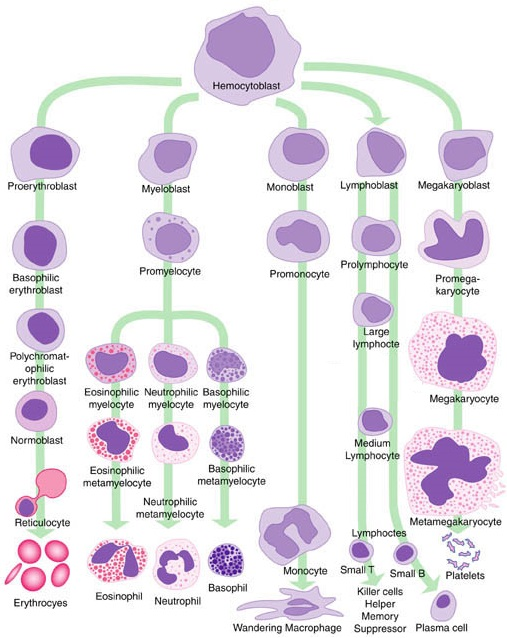
\includegraphics[width=0.98\textwidth]{images/Hematopoiesis}
	\caption{\label{fig:Haematopoiesis} Hematopoietic process.}
\end{figure}

\section{Granulopoiesis}
\textit{Granulocytes} are also called \textit{polymorphonuclear leukocytes} because of their characteristically shaped nuclei and cytoplasmic granules. Granulocytes include neutrophils, eosinophils, and basophils. A granulocyte differentiates into a distinct cell type by a process called granulopoiesis. The stages of maturation for the neutrophilic, eosinophilic and basophilic series is very similar. They start to differentiate at the third stage, so the first two stages are in common. The first five stages of granulopoiesis are illustrated in Fig.~\ref{fig:Granulopoiesis}.

\begin{figure}[!htbp]
	\centering
	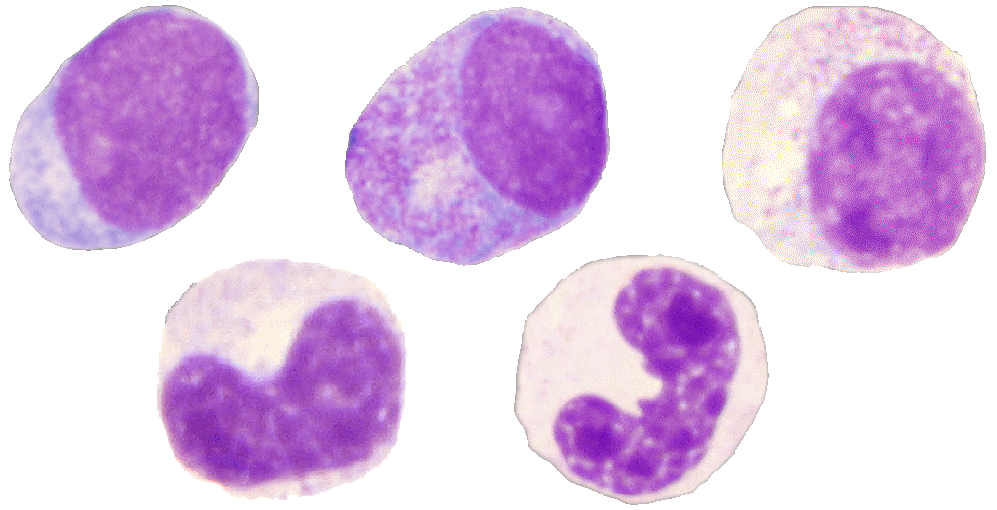
\includegraphics[width=0.88\textwidth]{images/granulopoiesis}
	\caption{\label{fig:Granulopoiesis} Granulopoiesis.}
\end{figure}

At the first stage of maturation the myeloid progenitor, called \textit{myeloblast}, has a size that ranges from 10 to 20 micron. The nucleus is large and centrally round, that could have a round or oval shape, and it has an open, unclumped nuclear chromatin that is of a light red-purple color. The nucleus contains several nucleoli, from two to five, which appear as lightened, refractile round structures, while the cytoplasm is weak and has a moderate blue color and usually without granules. At the second stage the myeloblast transforms in a \textit{promyelocyte} or \textit{progranulocyte}, that has a similar size that ranges from 10 to 22 micron. The nucleus is oval, round, or eccentric and the nuclear chromatin is more condensed of a light red-purple color. The nucleus contains less prominent nucleoli while the cytoplasm presents azurophilic granules. At this stage, the three series starts to differentiate, even if they preserve a similar appearance. Thus the promyelocyte gives rise to a unique myelocyte that can either be eosinophilic, basophilic, or neutrophilic.
The myelocyte then differentiates further into a metamyelocyte and then into a band cell before becoming a mature neutrophil, eosinophil, or basophil. The \textit{myelocytes} are slightly smaller than promyelocytes with a diameter of 10-18 micron. They present an eccentric, round-oval nucleus with a coarse and condensed chromatin and small, non-visible nucleoli. Some azurophilic granules persist in the cytoplasm, but secondary or specific granules begin to predominate, in particular, the neutrophilic granules are dusty, subtle, and red-blue, while eosinophilic granules are large red-orange and singular, instead basophil granules are large deep blue-purple. The \textit{metamyelocytes} are slightly smaller than myelocytes with a diameter of  10-15 micron. They have characteristic kidney-shaped nuclei and relatively densely clumped nuclear chromatin with no nucleoli. The cytoplasm range from pale blue to pinkish and becomes filled with predominantly secondary granules, although primary granules persist, and tertiary granules begin to appear. The \textit{band forms} have a size of 9 to 15 micron, with a curved or band-shaped nucleus but non-lobular or unsegmented. The cytoplasm is brown-pink, with many fine specific or secondary granules, that start to predominate. The \textit{segmented forms} have a size similar to the band forms, but they present a segmented nucleus, with two to five nuclear lobes connected by thin threadlike filaments. The cytoplasm is pale lilac with blue shading and many fine secondary dust-like granules. In detail, \textit{neutrophils} or polymorphonuclear neutrophils have a diameter of 12-15 micron filled with pink or purple granules and 2-5 nuclear lobes. The chromatin of the segmented neutrophil is coarsely clumped. The cytoplasm is faint pink, and it is filled with fine pink secondary granules. They are involved in the defense against infections. Neutrophils are the most abundant white blood cells in humans and account for approximately 70\% of all white blood cells. The presence of abnormally low number of neutrophils is described as neutropenia. Also, the number of lobes and the extent of granulation are diagnostic. Neutrophils with more than 5 lobes are called hypersegmented neutrophils. Neutrophils with more intensely stained (large dark blue) and more granules are described as toxic granulated neutrophils. Vacuoles appear as holes in the cytoplasm and are frequently found in association with toxic granulation. \textit{Eosinophils} instead have a diameter of 10-15 micron and they are easily recognized in stained smears because of their cytoplasm is filled with large, red-orange granules and a bi-lobed nucleus. They are generally low in number (1-3\%). The presence of abnormally high number of eosinophils is described as eosinophilia. Also \textit{basophils} have a diameter of 10-15 micron and a coarse, clumped bi-lobed nucleus and the presence of many large, specific secondary purple-black granules in the cytoplasm. Basophils are the least often seen type of WBC (1\%). Increased basophils number is called basophilia.

Because white blood cells have such a short time span in the peripheral circulation, alterations either in quantity or in the quality of a particular white blood cell can be quite dramatic. As white blood cells increase, the peripheral smear usually shows an increased number of segmented neutrophils or the presence of younger cells. In either of these cases, toxic changes, such as toxic granulation, toxic vacuolization, the presence of Dohle bodies or Auer Bodies, Pelger-Huet and Hypersegmentation may be observed. These toxic changes are illustrated in Fig.~\ref{fig:Changes}.


\begin{figure}[!htbp]
	\centering
	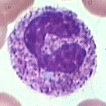
\includegraphics[width=0.15\textwidth]{images/granul}
	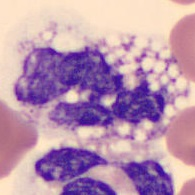
\includegraphics[width=0.15\textwidth]{images/vacuol}
	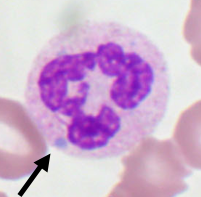
\includegraphics[width=0.15\textwidth]{images/Dohle}
	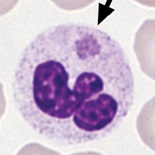
\includegraphics[width=0.15\textwidth]{images/Auer}
	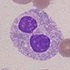
\includegraphics[width=0.15\textwidth]{images/Pelger}
	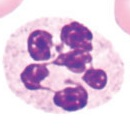
\includegraphics[width=0.15\textwidth]{images/hyper}
	\caption{\label{fig:Changes} Granulocyte toxic changes.}
\end{figure}

\textit{Toxic granulation} is excessive in amount and intensity, with more prominent granules in segmented neutrophils and bands. Normal granulation in the segmented neutrophils has a dust-like appearance, with the red and blue granules being challenging to observe, while, with toxic granulation, these granules are more frequent and have much more vivid blue-black coloration. Clusters of toxic granules usually appear in neutrophils. Sometimes the granulation is so dense as to resemble basophilic granules. Toxic granulation can be observed during acute bacterial infections. \textit{Toxic vacuolization} occurs in the segmented neutrophil with the appearance of small or large vacuoles in the cytoplasm. \textit{Dohle bodies} are light blue cytoplasmic inclusions that range from 1 to 5 micron in size, are located in the peripheral cytoplasm of neutrophils and appear as a rod-shaped, pale bluish grey structure. They are nuclear remnants that are often seen in association with toxic granules and vacuoles. Dohle bodies may be present in sepsis or severe inflammatory responses. \textit{Auer Bodies} are clumps of azurophilic granular material that form elongated needles seen in the cytoplasm of leukemic blasts. They are unique, pink or red rod-shaped inclusions that are seen in very immature granulocytes in patients with acute non-lymphocytic leukemia. \textit{Pelger-Huet} is an anomaly characterized by impaired nuclear segmentation of mature granulocytes. The nucleus is often in the shape of a peanut or dumbbell or may consist of two lobes connected with a filament. \textit{Hypersegmentation} is defined as a segmented neutrophilic nucleus having more than five lobes, since normal segmented neutrophils have between three and five lobes in the nucleus. 

\section{Monopoiesis}
The cell precursors called monoblasts produce monocytes. Monocytes differentiate and mature from monoblasts into promonocytes and then to matured monocytes. The stages of monopoiesis are illustrated in Fig.~\ref{fig:Monopoiesis}.

\begin{figure}[!htbp]
	\centering
	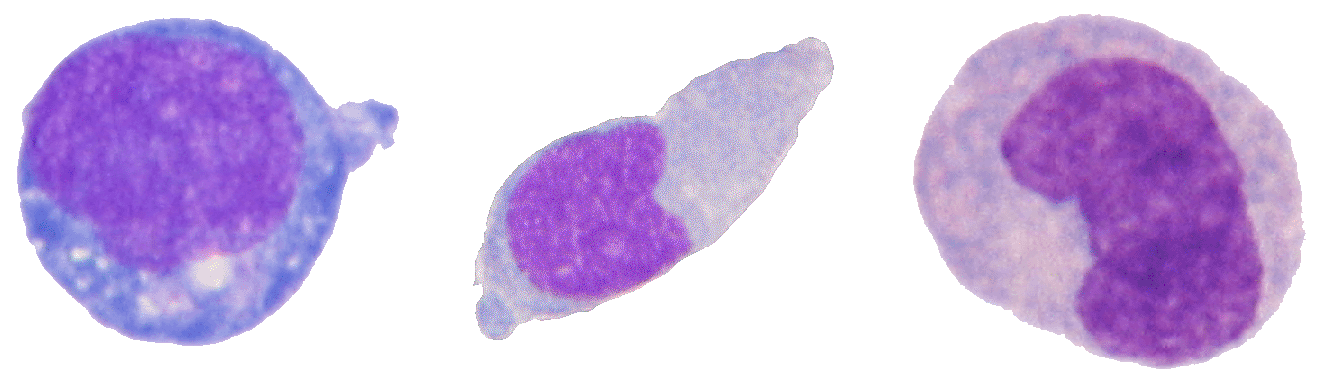
\includegraphics[width=0.88\textwidth]{images/monopoiesis}
	\caption{\label{fig:Monopoiesis} Monopoiesis.}
\end{figure}

\textit{Monoblast} is very similar to myeloblast, with a size of about 12-20 micron. The cytoplasm is agranular and the nucleus is large, round to oval and has fine nuclear chromatin. The main difference with myeloblast is that nucleoli (one or two) are more prominent in monoblasts. \textit{Promonocyte} has an average diameter of 14-18 micron. It has a large, convoluted nucleus, a coarse chromatin structure and one or two nucleoli. The cytoplasm is grey-blue and may contain a few fine azurophilic granules. \textit{Monocytes} are the largest of the white blood cells with a size of 12-20 micron. The cytoplasm is grey-blue, it may have numerous vacuoles and fine azurophilic granules. Monocytes have abundant cytoplasm and a large, distinctive, kidney-shaped nucleus. They circulate in the bloodstream for about one to three days, where they move into tissues throughout the body. They constitute between 3-8\% of all leukocytes in the blood. In the tissues, monocytes mature into different types of macrophages and help protect tissues from foreign substances. A decreased percentage of monocyte levels is called monocytosis.

\section{Lymphopoiesis}
Outlining the lymphocyte cell population is a complex task and beyond the scope of this thesis. Furthermore, some populations of lymphocytes appear morphologically similar to peripheral smear. For this reason, only a modified subset of sub-population is included. Lymphocytes are produced by the cell precursors called lymphoblast, that gives rise to prolymphocyte that differentiate into large lymphocyte and small lymphocyte.
Fig.~\ref{fig:Lymphopoiesis} shows the lymphocyte precursors.

\begin{figure}[!htbp]
	\centering
	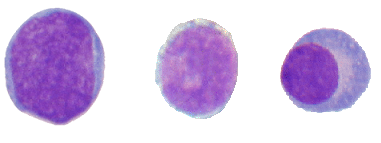
\includegraphics[width=0.78\textwidth]{images/lymphopoiesis}
	\caption{\label{fig:Lymphopoiesis} Lymphopoiesis.}
\end{figure}

\textit{Lymphoblasts} have a size of 10-20 micron with a little cytoplasm deep blue staining at the edge. They present one or two nucleoli. Prolymphocytes have a size of 9-18 with a grey-blue cytoplasm that is mostly blue at edges. The nucleus is almost round with coarse chromatin and some nucleoli may be present. \textit{Large lymphocytes} have a size of 15 to 18 micron, chromatin more transparent and they present a more significant amount of cytoplasm, lighter in color. \textit{Small lymphocytes} have a size of 7-12 micron. They present an oval eccentric nucleus with coarse, lumpy chromatin with specific areas of clumping.
The cytoplasm is usually just a thin border, with few azurophilic granules. Small lymphocytes consist of T cells and B cells, but it is not possible to distinguish between them in a peripheral blood smear as they appear morphologically similar. Their derivation and function, however, are entirely different. B lymphocytes comprise 10\% to 20\% of the total lymphocyte population, whereas T lymphocytes comprise 60\% to 80\%. A third minor population, NK lymphocytes, constitutes less than 10\% of the total lymphocyte population. Lymphocytes can also differentiate into dendritic cells, that unlike T-cells, B-cells and NK cells, arise from lymphoid or myeloid lineages. Lymphocytes frequently represent 20 to 40\% of circulating white blood cells, and they are the cornerstones of the adaptive immune system. T lymphocytes and B lymphocytes play a role in the maintenance of cell-mediated and antibody-mediated immunity. The increase in the number or proportion of lymphocytes in the blood is termed lymphocytosis, while a decreased number of lymphocytes is termed lymphocytopenia, or lymphopenia.

\section{Erythropoiesis}
Erythropoiesis is the process by which red blood cells (RBCs) or erythrocytes are produced. This process starts with the proliferation and differentiation of HSCs into the red cell precursors. This process is composed of six stages of maturation in the red blood cell series: pronormoblast, basophilic normoblast, polychromatophilic normoblast, orthochromatic normoblast, reticulocyte, and mature erythrocytes. In general, several morphological clues mark the RBC maturation series, the cell size decreases, nuclear chromatin becomes more condensed, the cytoplasm color is altered during hemoglobin production, but the most evident is the vanishing of the nucleus and the decrease in size, as it can be seen in Fig.~\ref{fig:Erythropoiesis}.

\begin{figure}[!htbp]
	\centering
	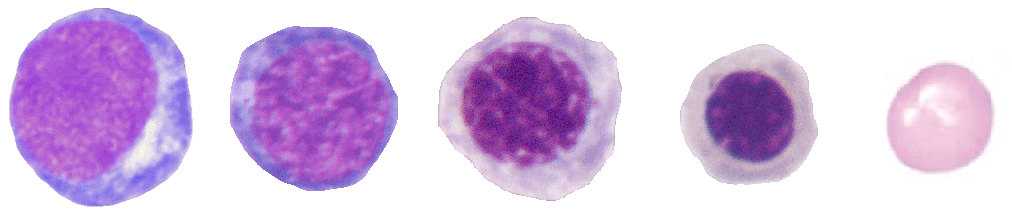
\includegraphics[width=0.98\textwidth]{images/erythropoiesis}
	\caption{\label{fig:Erythropoiesis} Erythropoiesis.}
\end{figure}

The \textit{proerythroblast} or \textit{pronormoblast} is typically 14-20 micron in size. It presents a round centrally located nucleus with coarser chromatin, more reticular, and condensed with a fine texture with deep violet color, nucleoli may be present but are hard to visualize. The cytoplasm presents a dark marine blue color with definitive areas of clearing. The \textit{basophilic normoblast} or \textit{erythroblast} is slightly smaller in size then pronormoblast, typically 12-17 micron of diameter. The nucleus is round with crystalline chromatin appearance, and it presents closed nucleoli. The cytoplasm becomes more basophilic, a cornflower blue color with indistinct areas of clearing and a grainy and reticular textured chromatin. The \textit{polychromatic} or \textit{intermediate normoblast} has a size of 12-15 micron. The nuclear chromatin is condensed and moderately compacted with no nucleoli.
The nucleus becomes smaller with a size of 7-9 micron and the cytoplasm color shift from deep basophilic to grey. The \textit{orthochromic} or \textit{non-nucleated normoblast} has a size of 8-12 micron. The cytoplasm increases with orange-red color tinges with slight blue tone. The nuclear chromatin condenses further, and the nucleus shrinks and tends to become more peripheral and eventually extruded. An orthochromatic normoblast becomes a reticulocyte once the nucleus is extruded. \textit{Reticulocytes} or \textit{polychromatic erythrocyte} are larger about twice than normal mature red cells, with a size of 8 microns, but the most evident difference is the presence of a reticulum in the cytoplasm.
The mature cell is released from the bone marrow into peripheral circulation at the reticulocyte stage. Under normal circumstances, reticulocytes constitute about 1\% of circulating red blood cells. The reticulocyte count is the most effective measure of erythropoietic activity since it reflects bone marrow healthy or injured. Low reticulocyte counts indicate decreased erythropoietic activity or may occur in ineffective erythropoiesis, a condition in which red blood cell precursors are destroyed before they are delivered to the peripheral circulation, or if the bone marrow is infiltrated with a tumor or abnormal cells. Increased reticulocyte counts indicate increased erythropoietic activity, usually as the bone marrow compensates in response to anemia. The reticulocyte matures after one to two days in circulation into a mature and functional RBC. The mature \textit{erythrocytes} present a significant reduction in the cell size that ranges from 6 to 8 micron and the cytoplasm changes characteristically from blue to salmon pink. Erythrocytes are disk-shaped cells, due to the presence of hemoglobin that is located peripherally, leaving an area of central pallor equal to 1-3 micron, approximately 30-45\% of the diameter of the cells. 

\subsection{Erythrocyte Variations}
Identifying normal and abnormal erythrocytes is important since automated cell counters have not yet replaced the well-trained eye with respect to the subtleties of red blood cell morphology. Erythrocytes of average size are termed \textit{normocytes}, while erythrocytes larger than average, thus with a diameter greater than 9 microns, are called \textit{macrocytes}, while smaller than average, thus with a diameter less than 6 microns, are called \textit{microcytes}. Erythrocyte color, that in normal conditions is pinkish red with central pallor, is representative of hemoglobin concentration in the cell. Under normal conditions, when the color, central pallor, and hemoglobin are proportional, the erythrocyte is termed \textit{normochromic}. \textit{Hypochromic} cells exhibit an area of central pallor larger than average, thus greater than 50\% of the diameter (3 microns), that means a decreased hemoglobin concentration. \textit{Polychromatophilic} cells exhibit a blue-grey cytoplasm, and they are slightly larger than average. Poikilocytosis is a general condition associated with the presence of one or more types of abnormally shaped mature erythrocytes, some of which may indicate the possible presence of a specific disease or disorder. Examples include; spherocytes, elliptocytes, sickle cells, teardrop cells, echinocytes, acanthocytes, keratocytes, bite cells, schistocytes, target cells, stomatocytes, and rouleaux formation. These shape abnormalities are illustrated in Fig.~\ref{fig:Poikilocytosis}.

\begin{figure}[!htbp]
	\centering
	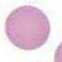
\includegraphics[width=0.15\textwidth]{images/spherocyte}\vspace{1mm}
	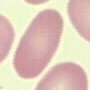
\includegraphics[width=0.15\textwidth]{images/Ovalocyte}
	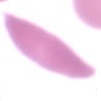
\includegraphics[width=0.15\textwidth]{images/sickle}
	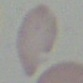
\includegraphics[width=0.15\textwidth]{images/Tear}
	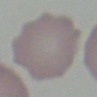
\includegraphics[width=0.15\textwidth]{images/Echinocyte}
	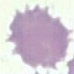
\includegraphics[width=0.15\textwidth]{images/Acanthocyte}
	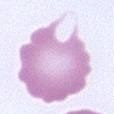
\includegraphics[width=0.15\textwidth]{images/keratocyte}
	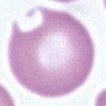
\includegraphics[width=0.15\textwidth]{images/bite}
	
\includegraphics[width=0.15\textwidth]{images/schistocyte}
	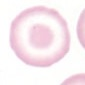
\includegraphics[width=0.15\textwidth]{images/Target}
	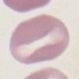
\includegraphics[width=0.15\textwidth]{images/Stomatocyte}
	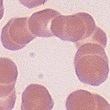
\includegraphics[width=0.15\textwidth]{images/reulex}
	\caption{\label{fig:Poikilocytosis} Poikilocytosis.}
\end{figure}

\textit{Spherocytes} are compact, round, densely staining red cells that lack central pallor. They are easily recognized among the rest of the red blood cell because they are dense, dark and small. \textit{Ovalocytes} or \textit{elliptocytes} are the most common red cells. They appear rather than the typical biconcave disc-shaped. Erythrocytes with this defect range from slightly oval to elongated cigar-shaped forms and they may appear macrocytic, hypochromic, or normochromic.  \textit{Sickle cells} are elongated or shaped like crescents or sickles. The fragile, sickle-shaped cells deliver less oxygen to the body's tissues. They can also get stuck more easily as they try to go through small blood vessels, and break into pieces that interrupt healthy blood flow. Many sickle cells may revert to normal disk shape on oxygenation, but approximately 10\% are unable to revert.
\textit{Teardrop} are characterized by a smaller size and above all from the appearance that resembles a tear. \textit{Acanthocytes} are characterised by a smaller size and above all from the presence of thorny projections distributed irregularly around the red blood cell, which lacks central pallor. The number of thorn can range from three to nine and must be distinguished from the \textit{echinocytes}, in which the projections are typically evenly spaced on the cell surface and they are more numerous, from 10 to 30. Another difference is that echinocytes have serrated edges over the entire surface and often the membrane is smaller and much more uniform in shape and distribution. \textit{Schistocytes} are fragmented erythrocytes  that are irregular in shape and size. They are usually half the size of the normal red blood cells and have a deeper red colour. They can appear as small triangular erythrocytes, helmet cells, and normal-size erythrocytes with 2 to 3 pointed surface  projections (\textit{keratocytes}). Round erythrocytes with a single, elliptical or round surface defect are termed \textit{bite cells}. \textit{Stomatocytes} are characterized by a mouth-shaped area of central pallor and a decrease in the ratio of surface area-to-volume that can be induced either by a reduction in surface area or an increase in red cell volume. Several agents can induce this morphology and often they can also be found on the peripheral smear of healthy subjects, due to drying artifact. It can be distinguished since the percentage of stomatocytes in healthy subjects is usually below 3\% of the total red cells. \textit{Target cells} have a centrally located disk of haemoglobin surrounded by an area of pallor with an outer ring of haemoglobin adjacent to the cell membrane giving the cell the appearance of a target. They are seen in the peripheral blood due to the presence of artefacts, because of decreased volume or increased red blood cell surface membrane. \textit{Rouleaux} formation is a phrase denoting an agglomerate of erythrocytes, that create a stack generally in a curving pattern. The flat surface of the RBCs give them a large surface area to make contact and stick to each other forming a rouleaux. 

\subsection{Erythrocyte Inclusions}
The cytoplasm of all normal red blood cells is free of debris, granules, or other structures. Inclusions are the result of unique conditions, and their identification can be clinically helpful. Examples of inclusion bodies are howell-jolly bodies, siderotic granules, basophilic stippling, Heinz bodies, malaria, and nucleated red cells. This cell inclusion is illustrated in Fig.~\ref{fig:Inclusions}.

\begin{figure}[!htbp]
	\centering
	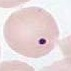
\includegraphics[width=0.15\textwidth]{images/Howell}
	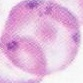
\includegraphics[width=0.15\textwidth]{images/siderotic}
	
\includegraphics[width=0.15\textwidth]{images/basophilic}
	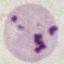
\includegraphics[width=0.15\textwidth]{images/Heinz}
	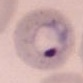
\includegraphics[width=0.15\textwidth]{images/Malaria}
	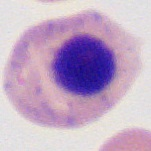
\includegraphics[width=0.15\textwidth]{images/nucleated}
	\caption{\label{fig:Inclusions} Erythrocyte Inclusions.}
\end{figure}

\textit{Howell-jolly bodies} represent remnants of the nucleus as it is extruded from the cytoplasm, that appears in the red blood cell as round, deep purple structures of about 1 micron in size. They are eccentrically located in the cytoplasm and seen when erythropoiesis is rushed. \textit{Siderotic granules} or \textit{Pappenheimer bodies} appear as small, dark blue or purple dots, located along the periphery of the red blood cells. \textit{Basophilic stippling} refers to numerous tiny coarse or fine blue granules in the periphery of the cytoplasm. They are difficult to visualize in the peripheral smear without fine focusing, but red blood cell containing basophilic stippling often is polychromatophilic. \textit{Heinz bodies} are defined as large structures approximately 1 to 3 micron in diameter located toward the periphery of the red blood cell membrane. Although they cannot be visualized by standard stain, bite cells in the peripheral smear are evidence that a Heinz body has been formed. \textit{Malaria} is a mosquito-borne infectious disease that results from the multiplication of a parasite within the cytoplasm of the red blood cells. Five species of this parasite can infect and be transmitted by humans, for this reason, the inclusion appearance can be very different. \textit{Nucleated red blood cells} (NRBCs), that are red cells with a retained nucleus can be observed inside the blood smears. The average size of the NRBC is 7-12 micron in diameter, the cytoplasm is pink, and the nucleus is a homogeneous blue-black mass with no structure. NRBCs detection and quantification is still based on the microscopic analysis of stained blood, since they are often counted as white cells by most hematology analyzers because of the presence of the retained nucleus, and this, in particular in patients with a high nucleated cell count, could lead to misleading results. Sometimes platelets overlying erythrocytes may be mistaken for erythrocyte inclusions. 

\section{Megakaryocytopoiesis}
Megakaryocytopoiesis is the process by which platelets or thrombocytes are produced. Platelet development is originated in the bone marrow from the HSC that differentiate into the megakaryocytic precursor, that then develops into the megakaryoblast, that gives rise to the pro-megakaryocyte and then the megakaryocyte before developing into mature platelets. During this period the megakaryocyte nucleus undergoes extensive endomitosis, the cytoplasmic differentiation, the formation of platelet granules, and the fragmentation into mature platelets as it can be seen in Fig.~\ref{fig:Megakaryocytopoiesis}.

\begin{figure}[!htbp]
	\centering
	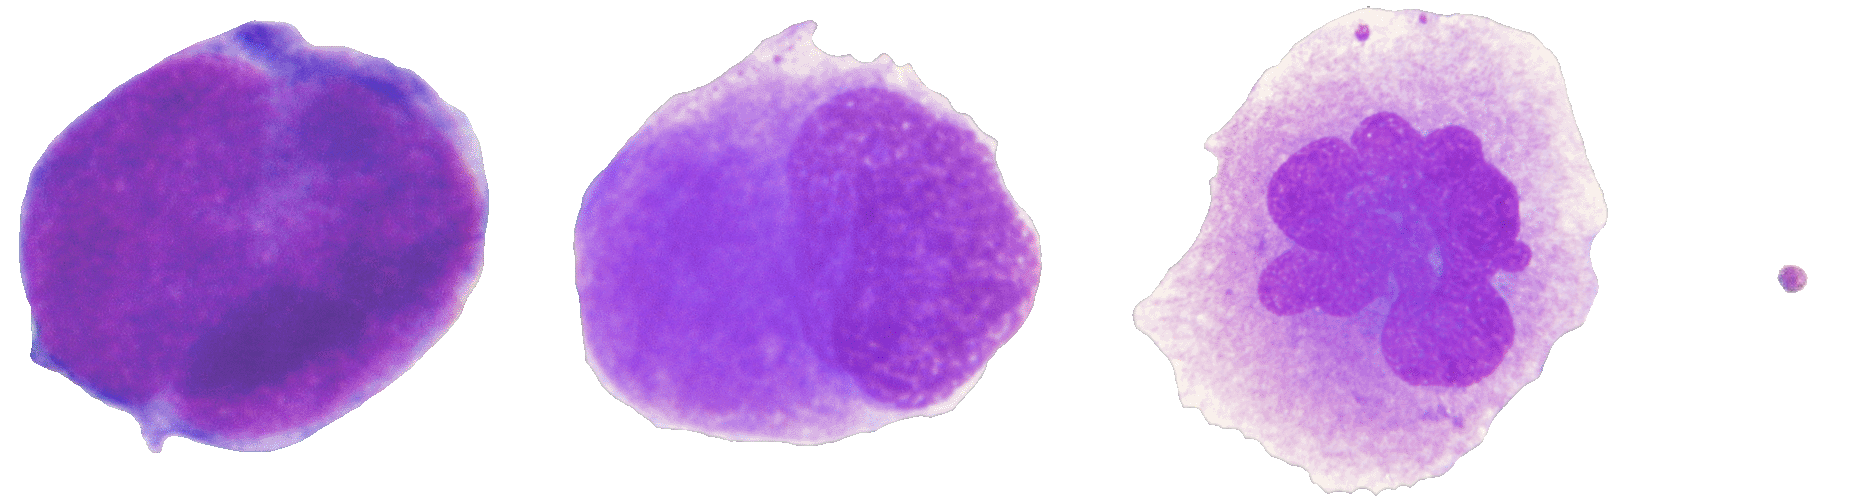
\includegraphics[width=0.98\textwidth]{images/megakaryopoiesis}
	\caption{\label{fig:Megakaryocytopoiesis} Megakaryocytopoiesis.}
\end{figure}

The \textit{megakaryoblast} has a size between 20 to 30 micron. Its nucleus is large, oval or kidney-shaped and contains several nucleoli. It has an insignificant non-granular and slightly basophilic cytoplasm. The \textit{pro-megakaryocyte} is very similar to the megakaryoblast except for the presence of an intensely basophilic cytoplasm that contains fine azurophilic granules. The \textit{megakaryocyte} instead is much bigger than its precursors, having a size around 50-100 micron. It presents a single, indented nucleus and a basophilic (light blue) cytoplasm that contains azurophilic granules.
Each megakaryocyte fragments into thousands of platelets. \textit{Platelets} are very small, about 3 microns, the cytoplasm is stained light blue, and it contains purple-reddish granules. Platelets play a crucial role in hemostasis, and they are involved in the formation of blood clot. A low number of platelets is called thrombocytopenia, while a decrease in function of platelets is called thrombasthenia. In some people, too many platelets may be produced, which may result in interferences with the flow of blood.
An increase in the number of platelets is called thrombocytosis. Sometimes this problem could cause bleeding, because many of the extra platelets may be dysfunctional even though they appear healthy. A platelet count is usually evaluated by preparing a blood smear to visualize any anomalies in shape or size directly. Blood smear could present platelets greater than 3 microns in diameter, that is called macrocytic platelets or megathrombocytes. The modern hematology analyzers disregard this kind of platelets since they count the platelets based on their sizing. Also, the count is falsely low when there are platelets clumps. In such instances, the instrument does not count these clumps of platelets and gives the platelet count as falsely low. Usually, in a healthy person, less than 5\% of the platelets appear large. Platelet size is of diagnostic significance, particularly if considered in relation to the platelet count. Small or normal-sized platelets in association with thrombocytopenia are suggestive of a failure of bone marrow production, while thrombocytopenia with large platelets is more likely to be caused by peripheral destruction or consumption of platelets with the bone marrow responding by increasing platelet production. Platelet size is also useful in assessing the likely cause of thrombocytosis. 

\section{Malaria parasites}
Human malaria infection is not strongly related to cell count, but it needs different tests to be identified. It can only be caused by parasitic protozoans belonging to the \emph{Plasmodium} type. The parasites are spread to people through the bites of infected female Anopheles mosquitoes, called~``malaria vectors''.
There are five parasite species that cause malaria in humans and two of these species, \emph{Plasmodium falciparum} and \emph{Plasmodium vivax}, constitute the greatest threat. \emph{Plasmodium~ovale}, \emph{Plasmodium malariae} and \emph{Plasmodium knowlesi} are the three remaining species that are less dangerous in humans \cite{WHO_dec_2016}, as shown in Figure \ref{fig:malaria_stages}.
All five species may appear in four different life-cycle stages during the infection phase in peripheral blood: ring, trophozoite, schizont, and gametocyte. Some~examples are shown in Figure \ref{fig:malaria_stages}.
The life-cycle-stage of the parasite is defined by its morphology, size and the presence or absence of malarial pigment.
The species differ in the changes of infected cell's shape, the presence of some peculiar dots and the morphology of the parasite in some of the life-cycle-stages~\cite{Somasekar2011}.
\begin{figure}[H]
	\centering
	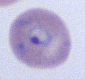
\includegraphics[width=2.5cm, height=2.5cm]{images/malaria/falciparum_1_ring}
	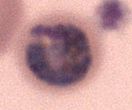
\includegraphics[width=2.5cm, height=2.5cm]{images/malaria/falciparum_2_trophozoiteAge}
	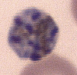
\includegraphics[width=2.5cm, height=2.5cm]{images/malaria/falciparum_3_schizont}
	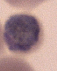
\includegraphics[width=2.5cm, height=2.5cm]{images/malaria/falciparum_4_gametocyte}
	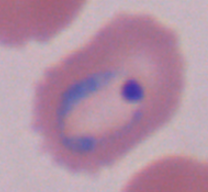
\includegraphics[width=2.5cm, height=2.5cm]{images/malaria/ovale_1_ring}
	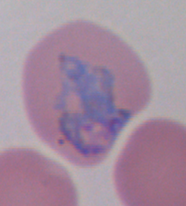
\includegraphics[width=2.5cm, height=2.5cm]{images/malaria/ovale_2_trophozoite}
	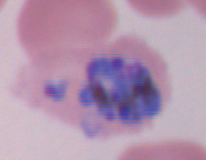
\includegraphics[width=2.5cm, height=2.5cm]{images/malaria/ovale_3_schizont}
	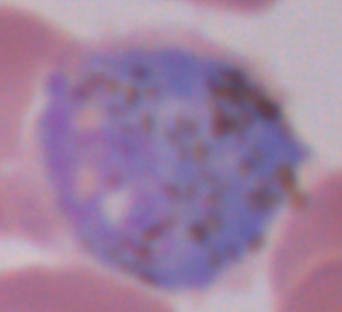
\includegraphics[width=2.5cm, height=2.5cm]{images/malaria/ovale_4_gametocyte}
	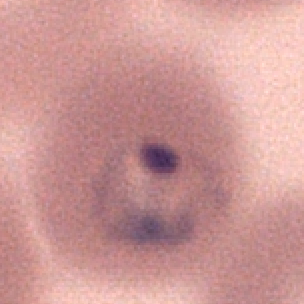
\includegraphics[width=2.5cm, height=2.5cm]{images/malaria/malariae_1_ring}
	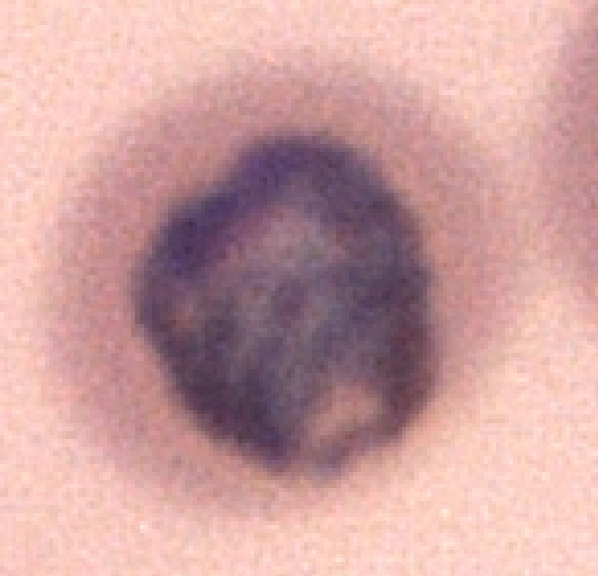
\includegraphics[width=2.5cm, height=2.5cm]{images/malaria/malariae_2_trophozoite}
	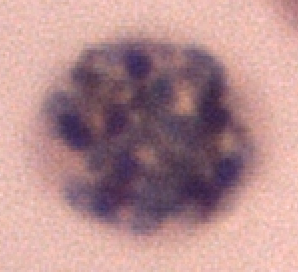
\includegraphics[width=2.5cm, height=2.5cm]{images/malaria/malariae_3_schizont}
	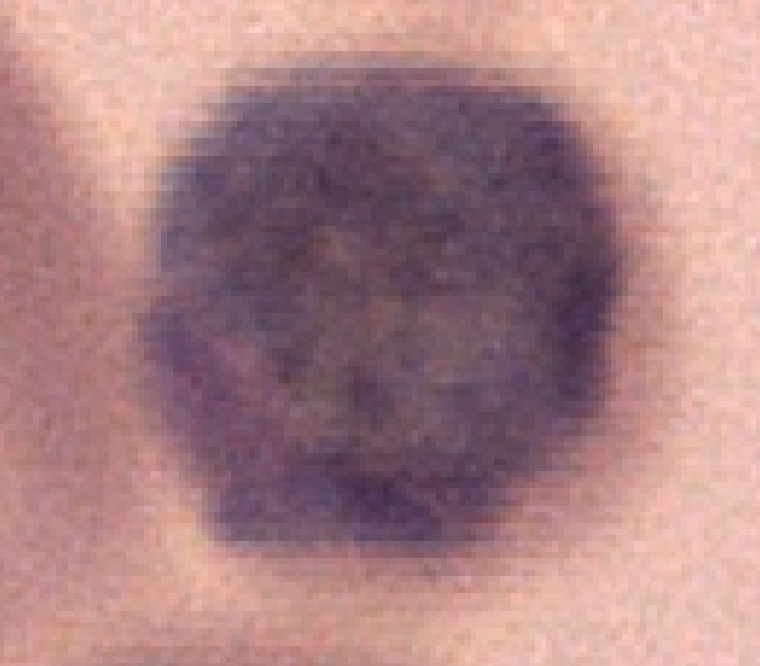
\includegraphics[width=2.5cm, height=2.5cm]{images/malaria/malariae_4_gametocyte}
	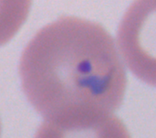
\includegraphics[width=2.5cm, height=2.5cm]{images/malaria/vivax_1_ring}
	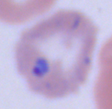
\includegraphics[width=2.5cm, height=2.5cm]{images/malaria/vivax_2c_trophozoiteDeveloped}
	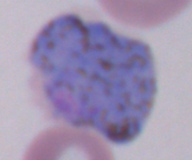
\includegraphics[width=2.5cm, height=2.5cm]{images/malaria/vivax_4_gametocyte}
	\caption[Malaria parasite stages.]{\label{fig:malaria_stages}Examples of malaria parasite stages.
		First row, from left to right: \emph{P. falciparum} ring, trophozoite, schizont, gametocyte;
		second row, from left to right: \emph{P. ovale} ring, trophozoite, schizont, gametocyte;
		third row, from left to right: \emph{P. malariae} ring, trophozoite, schizont, gametocyte;
		last row, from left to right: \emph{P. vivax} ring, developed trophozoite, gametocyte.
		Courtesy of CHUV, Lausanne.}
\end{figure}

Malarial parasite trophozoites are generally ring-shaped, 1-2 microns in size, although other forms (ameboid and band) may also exist. The sexual forms of the parasite (gametocytes) are much larger and 7-14 microns in size. P. Falciparum is the largest and is banana shaped while others are smaller and round. P. Vivax causes stippling of infected red cells.
\begin{figure}[!htbp]
	\centering
	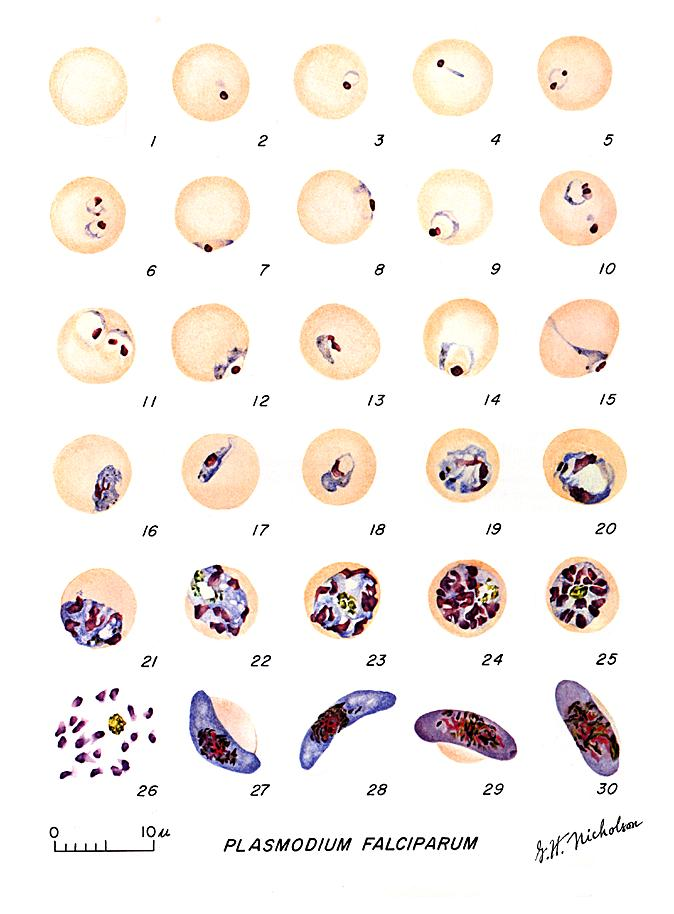
\includegraphics[width=0.90\textwidth]{images/malaria_th/mal_falc}
	\caption[Plasmodium Falciparum's stages of life.]{\label{fig:falci_th} Plasmodium Falciparum schematic stages of life. Courtesy of \cite{Med_cdc}.
		Fig. 1: Normal red cell; Figs. 2-18: Trophozoites (among these, Figs. 2-10 correspond to ring-stage trophozoites); Figs. 19-26: Schizonts (Fig. 26 is a ruptured schizont); Figs. 27, 28: Mature macrogametocytes (female); Figs. 29, 30: Mature microgametocytes (male).}
\end{figure}

\begin{figure}[!htbp]
	\centering
	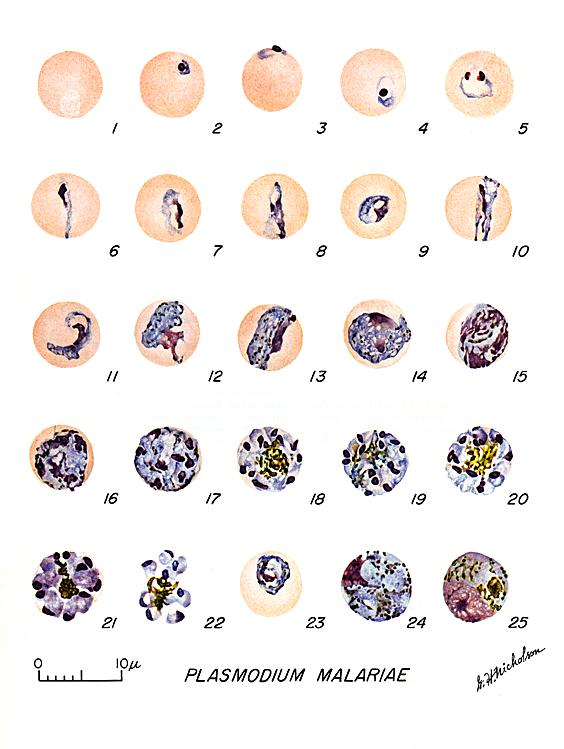
\includegraphics[width=0.90\textwidth]{images/malaria_th/mal_mal}
	\caption[Plasmodium Malariae's stages of life.]{\label{fig:mal_th} Plasmodium Malariae schematic stages of life. Courtesy of \cite{Med_cdc}.
		Fig. 1: Normal red cell; Figs. 2-5: Young trophozoites (rings); Figs. 6-13: Trophozoites; Figs. 14-22: Schizonts; Fig. 23: Developing gametocyte; Fig. 24: Macrogametocyte (female); Fig. 25: Microgametocyte (male).}
\end{figure}

\begin{figure}[!htbp]
	\centering
	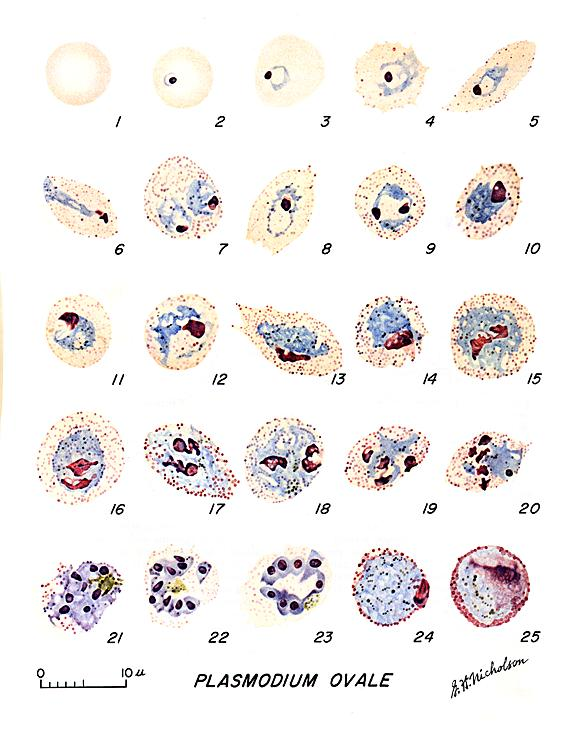
\includegraphics[width=0.98\textwidth]{images/malaria_th/mal_ova}
	\caption[Plasmodium Ovale's stages of life.]{\label{fig:ova_th} Plasmodium Ovale schematic stages of life. Courtesy of \cite{Med_cdc}.
		Fig. 1: Normal red cell; Figs. 2-5: Young trophozoites (Rings); Figs. 6-15: Trophozoites; 
		Figs. 16-23: Schizonts; Fig. 24: Macrogametocytes (female); Fig. 25: Microgametocyte (male).}
\end{figure}

\begin{figure}[!htbp]
	\centering
	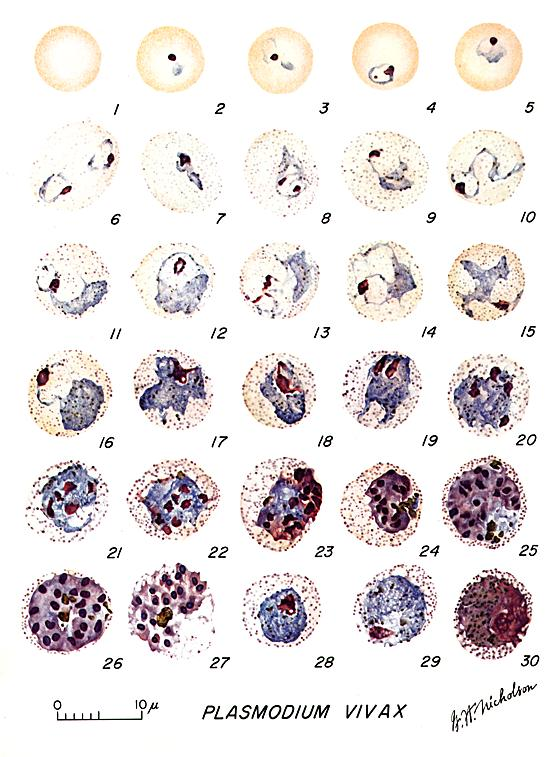
\includegraphics[width=0.90\textwidth]{images/malaria_th/mal_viv}
	\caption[Plasmodium Vivax's stages.]{\label{fig:vivax_th} Plasmodium Vivax schematic stages of life. Courtesy of \cite{Med_cdc}.
		Fig. 1: Normal red cell; Figs. 2-6: Young trophozoites (ring stage parasites); Figs. 7-18: Trophozoites; Figs. 19-27: Schizonts; Figs. 28 and 29: Macrogametocytes (female); Fig. 30: Microgametocyte (male).}
\end{figure}